\hypertarget{_project_description_ProjectDescriptionInstallations}{}\section{Installations}\label{_project_description_ProjectDescriptionInstallations}
The installers were uploaded on Source\+Forge \cite{sourceforge}. The download page is available at\+: \href{https://sourceforge.net/projects/dualstateframework/}{\tt https\+://sourceforge.\+net/projects/dualstateframework/}. Click the \char`\"{}files\char`\"{} tab, you will see all versions for different platform. 
\begin{DoxyImageNoCaption}
  \mbox{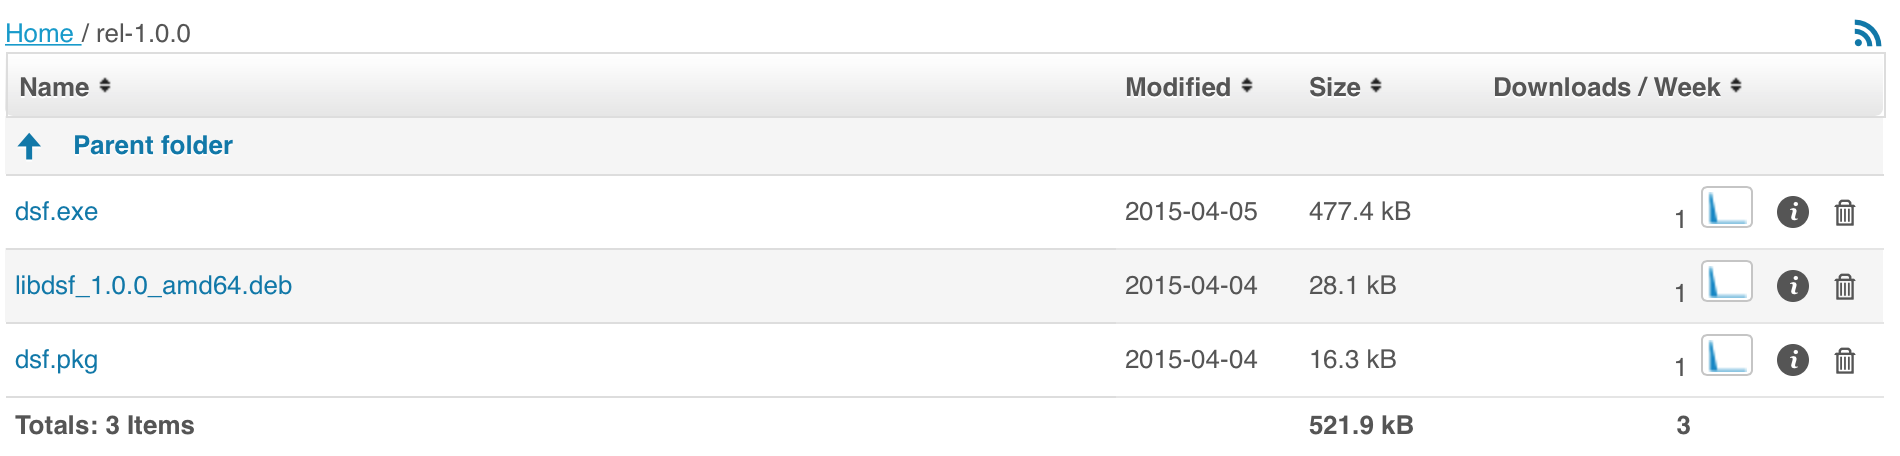
\includegraphics[width=\textwidth,height=\textheight/2,keepaspectratio=true]{ReportDescriptionInstallations.png}}
\end{DoxyImageNoCaption}
\hypertarget{_project_description_ProjectDescriptionFrameworkwithXcode}{}\section{Framework with Xcode}\label{_project_description_ProjectDescriptionFrameworkwithXcode}
The library is designed as a bundle \cite{bundle} for Mac O\+S X. To use it in Xcode you just need to drag it into your project explorer. 
\begin{DoxyImageNoCaption}
  \mbox{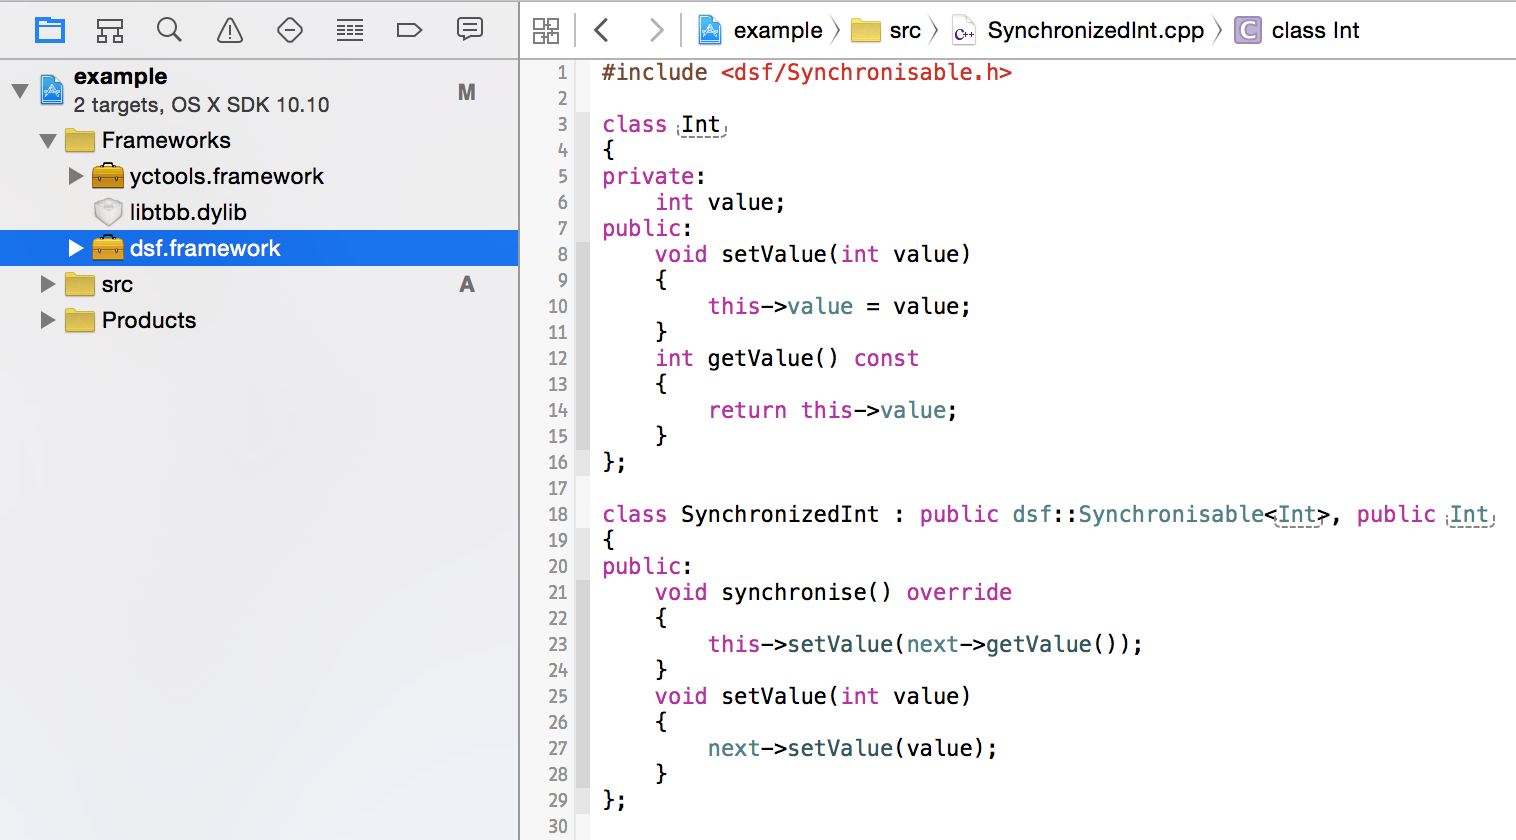
\includegraphics[width=\textwidth,height=\textheight/2,keepaspectratio=true]{ReportDescriptionXcode.png}}
\end{DoxyImageNoCaption}
\hypertarget{_project_description_ProjectDescriptionBenchmarkProgram}{}\section{Benchmark Program}\label{_project_description_ProjectDescriptionBenchmarkProgram}
The benchmark program is designed for profiling the library. It allows user to configure settings. 
\begin{DoxyImageNoCaption}
  \mbox{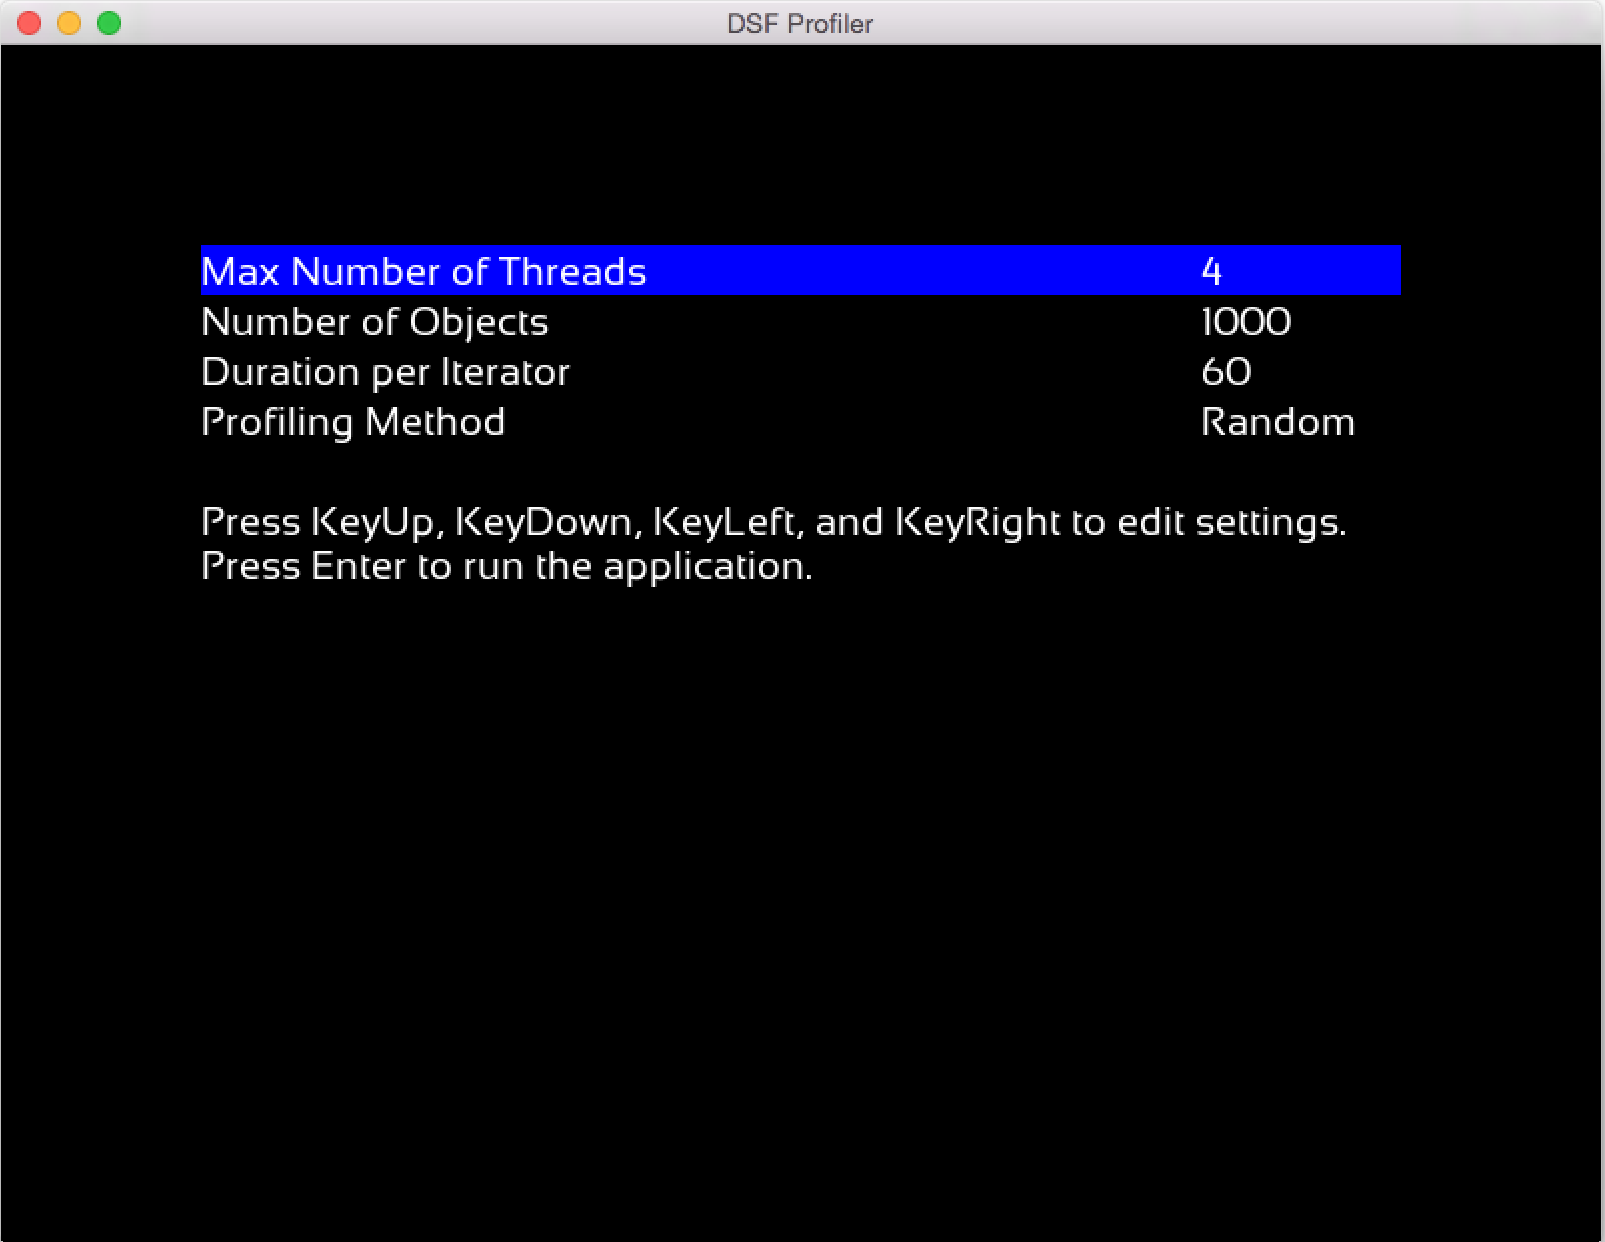
\includegraphics[width=12cm]{ReportDescriptionBenchmark.png}}
\end{DoxyImageNoCaption}
 While running it shows the maximum, minimum, and average F\+P\+S on the screen. 
\begin{DoxyImageNoCaption}
  \mbox{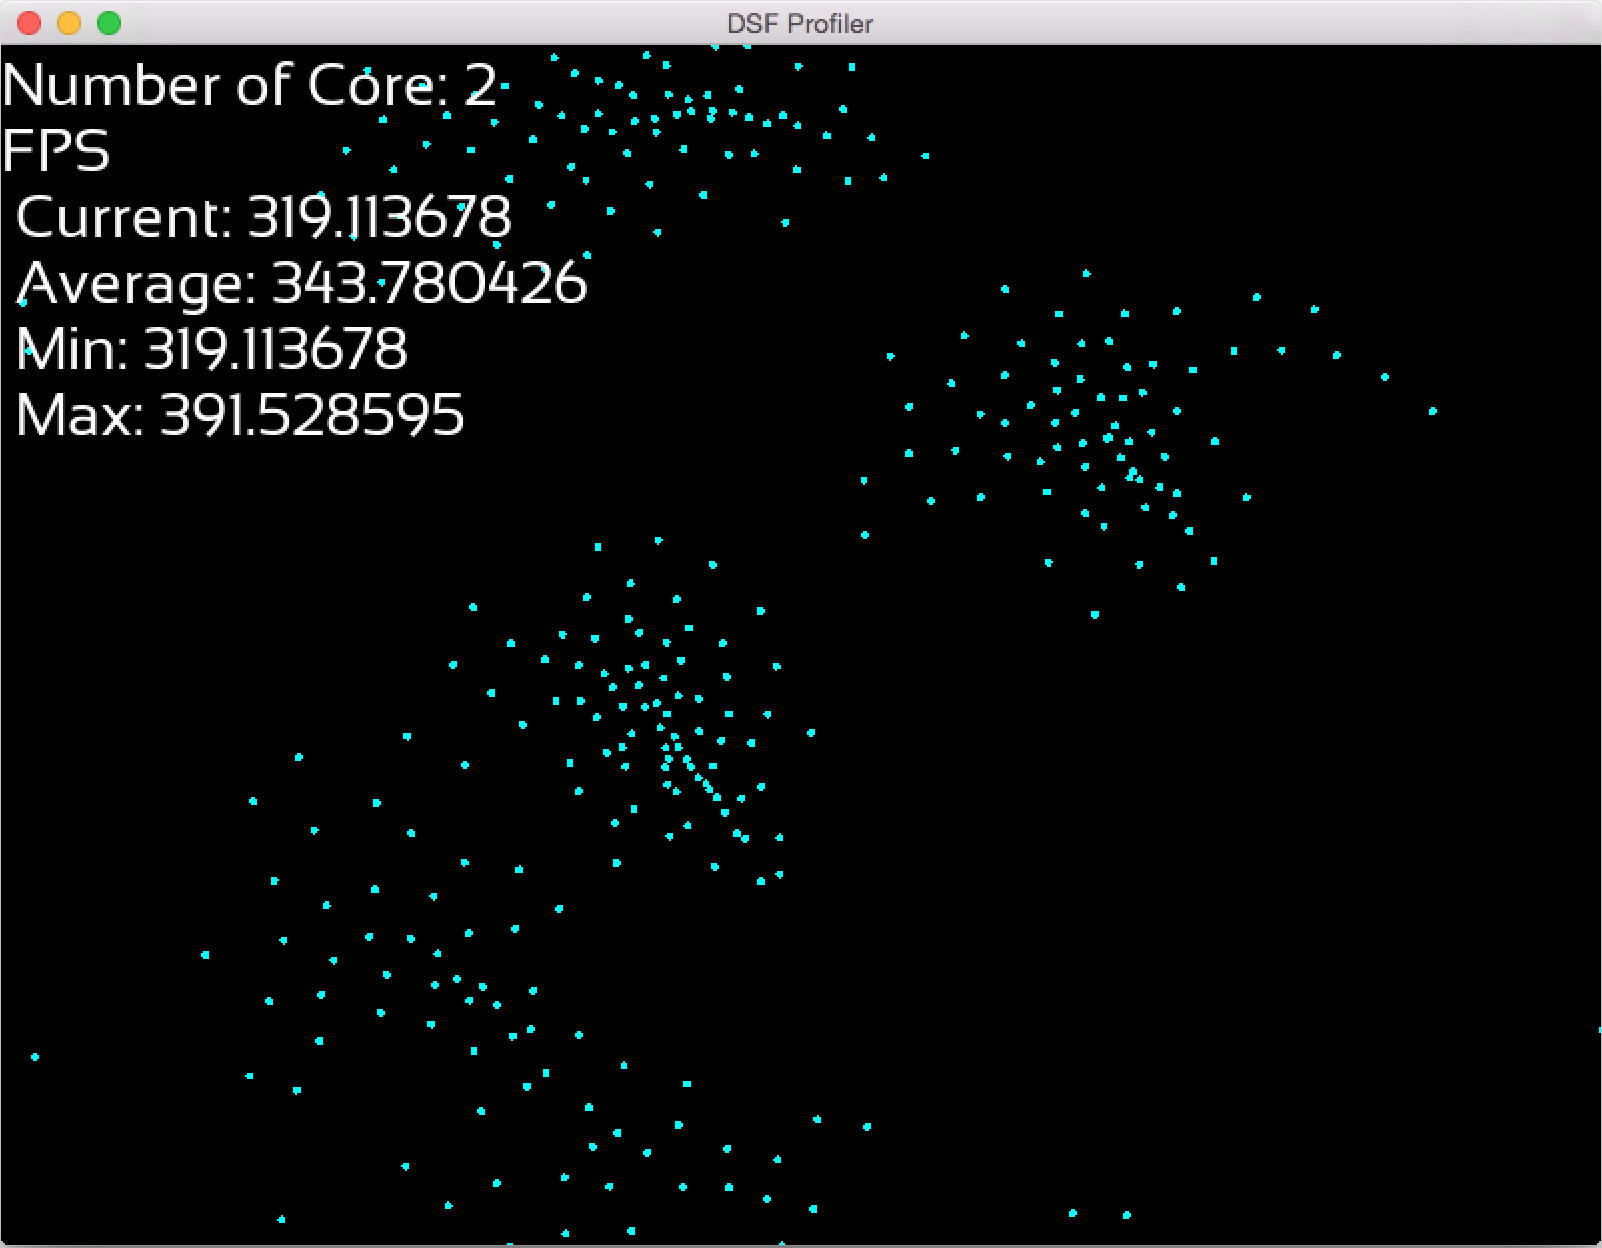
\includegraphics[width=12cm]{ReportDescriptionBenchmarkRunning.png}}
\end{DoxyImageNoCaption}
 The output is a bar graph. X axis is the number of threads, and y axis in the F\+P\+S. 
\begin{DoxyImageNoCaption}
  \mbox{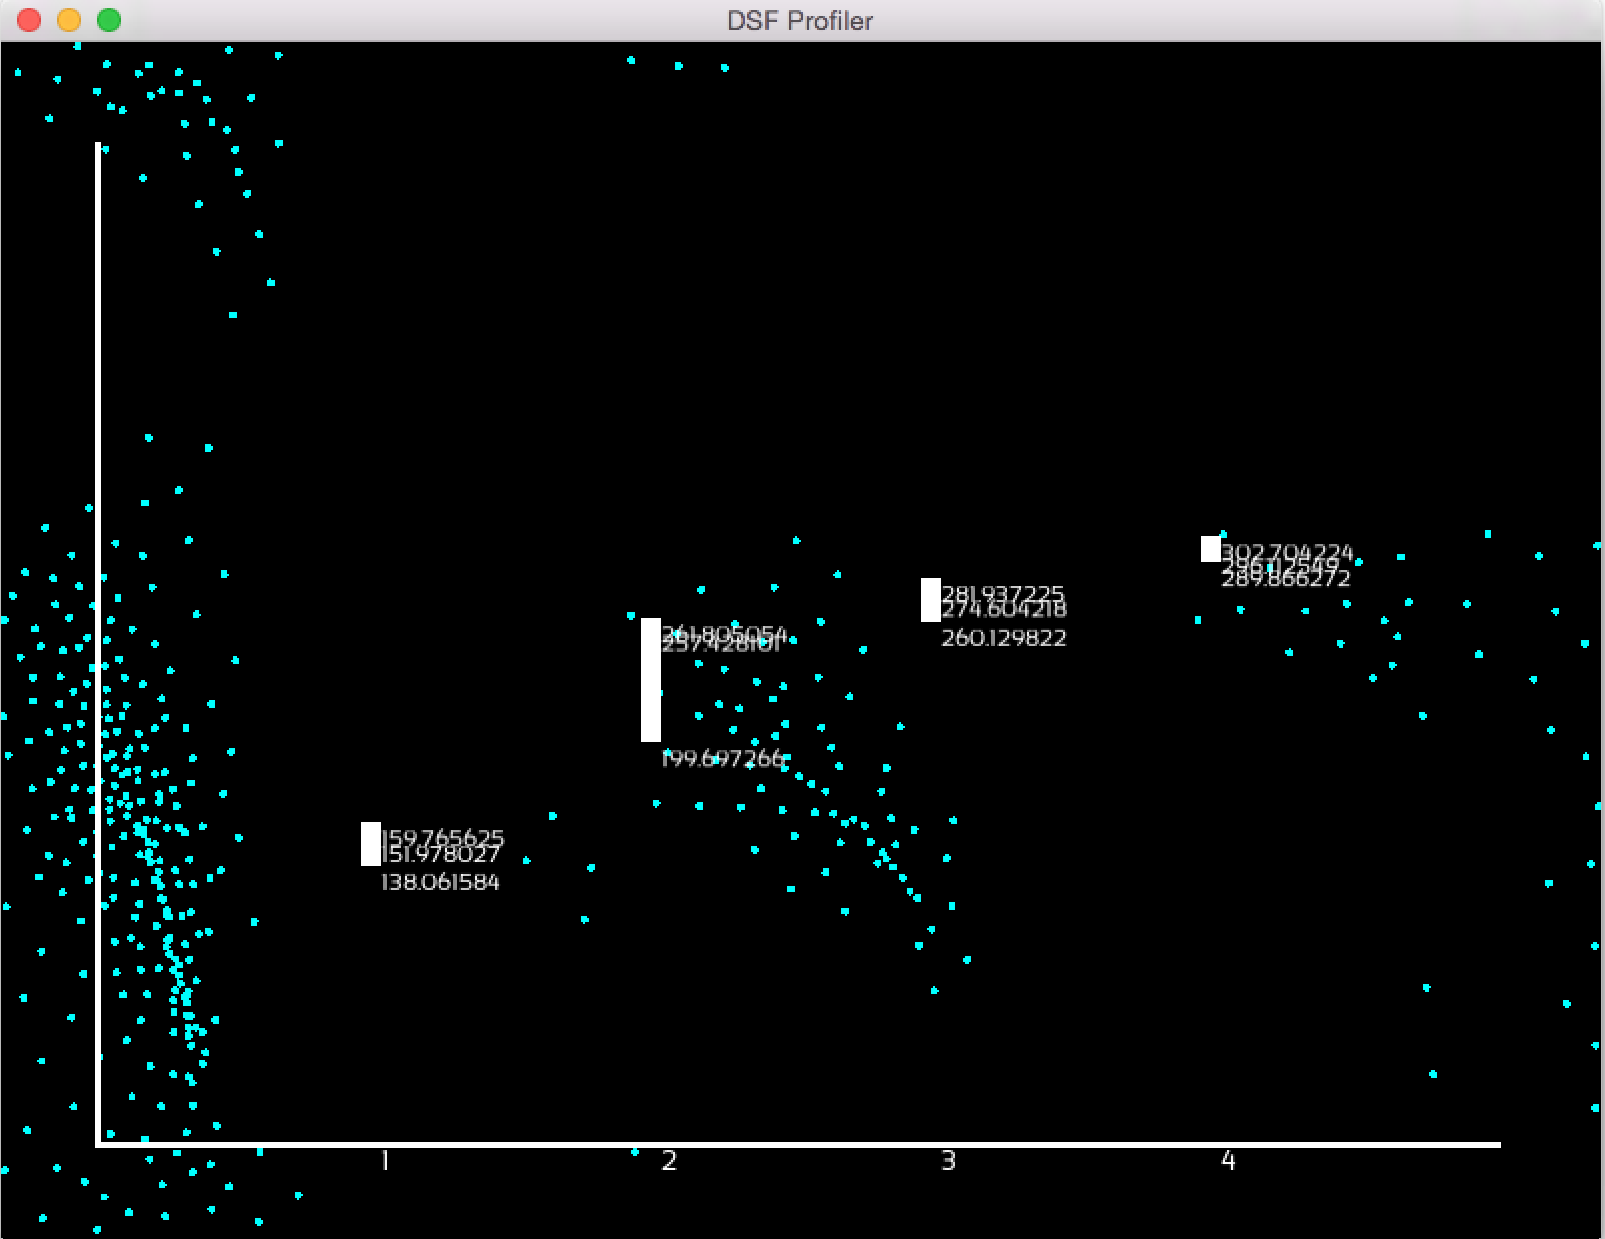
\includegraphics[width=12cm]{ReportDescriptionBenchmarkOutput.png}}
\end{DoxyImageNoCaption}
 